\documentclass[12pt,a4paper,oneside]{book}
\usepackage[utf8]{inputenc}
\usepackage{graphicx} %input gambar
\usepackage{amsmath}
\usepackage{amsfonts}
\usepackage{amssymb}
\usepackage{float}
%Mengatur ke font times new rouman
\usepackage{mathptmx}

\usepackage[T1]{fontenc}
%
\usepackage{pdfpages}

% Garis tepi (margin)
%\usepackage[paperheight=29.7cm,paperwidth=21cm]{geometry}
\usepackage{geometry}
 \geometry{
 left=4cm,
 top=4cm,
 right=3cm,
 bottom=3cm,
 }

% mengatur 1 cm baris pertama paragraf
\usepackage{indentfirst}
\setlength{\parindent}{1cm}

% Mengkompres cite
\usepackage[numbers]{natbib}

% Mengatur page number
\usepackage{fancyhdr}
\pagestyle{fancy}
\renewcommand{\headrulewidth}{0pt} %menghilangkan garis

% change name Daftar Isi, Daftar Pustaka jadi section
\renewcommand{\contentsname}{DAFTAR ISI}
\renewcommand{\chaptername}{BAB}
\renewcommand{\bibname}{DAFTAR PUSTAKA}
\renewcommand{\listfigurename}{DAFTAR GAMBAR}
\renewcommand{\figurename}{Gambar}
\renewcommand{\listtablename}{DAFTAR TABEL}
\renewcommand{\tablename}{Tabel}
\renewcommand{\appendixname}{Lampiran}

% change languange dan pemenggalan kata
%\usepackage[indonesian]{babel}
\sloppy %agar teks tidak lebih saat rata kanan kiri

% numbering
\renewcommand{\thechapter}{\Roman{chapter}} %Peringkat 1
\renewcommand{\thesection}{\Alph{section}.} %Peringkat 2
\renewcommand{\thesubsection}{\arabic{subsection}.} %Peringkat 3
\renewcommand{\thefigure}{\arabic{chapter}.\arabic{figure}}%gambar
\renewcommand{\thetable}{\arabic{chapter}.\arabic{table}}%tabel
\renewcommand{\theequation}{\arabic{chapter}.\arabic{equation}}%equestion

\setcounter{secnumdepth}{3}
\renewcommand{\thesubsubsection}{\thesubsection\arabic{subsubsection}}

% baris antar paragraf
\linespread{1.5}

% mengatur title section
\usepackage{titlesec}
\titleformat{\chapter}[display]   
{\centering\normalfont\large\bfseries}
{\MakeUppercase{\chaptertitlename}\ \thechapter}{0pt}{\large}   
\titlespacing*{\chapter}{0pt}{-50pt}{40pt}
% ukuran section dan subsection
\titleformat{\section}
  {\normalfont\fontsize{12}{15}\bfseries}{\thesection}{1em}{}
\titleformat{\subsection}
  {\normalfont\fontsize{12}{15}\bfseries}{\thesubsection}{1em}{}

% untuk modif numbering
\usepackage{enumitem}

% membuat link
\usepackage{hyperref}

%\usepackage{soul} %digunakan sementara untuk meng-highlight teks yang belum diubah

\usepackage[none]{hyphenat} %untuk menghilangkanpemenggalan kata

% Perlengkapan pada table
\usepackage{colortbl} %untuk color table
\usepackage{adjustbox} %agar table pas di halaman (tidak lebih)
\usepackage{longtable} %Untuk membuat table lebih panjang
\usepackage{multirow}

\usepackage{float} %digunakan agar gambar dan tabel tidak pindah, cara menggunakan dengan menambah [H]

% Untuk membuat flowchart
\usepackage{tikz}
\usetikzlibrary{shapes.geometric, arrows}

\usepackage{wrapfig} %untuk menambah wrap figure

% Untuk membuat subfigure, dan subtable
\usepackage[labelsep=space,labelfont=bf,font=bf]{caption} %menghilangkan titik dua (:), tebal pada caption gambar
\usepackage{subcaption}

\begin{document}

\newpage
\begin{titlepage}
   \begin{center}

       \textbf{PENERAPAN $K$-MEANS DAN ALGORITMA GENETIKA UNTUK MENYELESAIKAN MTSP}
       
       (Studi Kasus Pada Perjalanan Menuju Seluruh SMA di Kabupaten Probolinggo)

       \vfill
       \textbf{SKRIPSI}
       \vfill
       
       
\includegraphics[width=0.4\textwidth]{Gambar/logo.png}
       
       \vfill
       
       \textbf{OLEH:}\\
       \textbf{\underline{MUHAMMAD FAIZ NAILUN NI'AM}}\\
       NIM : 1842200034

       \vfill
       
       UNIVERSITAS NURUL JADID\\
       PAITON PROBOLINGGO\\
       \textbf{FAKULTAS SOSIAL DAN HUMANIORA}\\       
       PROGRAM STUDI PENDIDIKAN MATEMATIKA\\
       
       \vfill       
       
       AGUSTUS 2022
       
   \end{center}
\end{titlepage}

% Halaman depan
\newpage
\frontmatter
\begin{center}

\textbf{PENERAPAN $K$-MEANS DAN ALGORITMA GENETIKA UNTUK MENYELESAIKAN MTSP}
       
       (Studi Kasus Pada Perjalanan Menuju Seluruh SMA di Kabupaten Probolinggo) 
       
       \vfill
       \textbf{SKRIPSI}
       \vfill
       
       DIAJUKAN KEPADA UNIVERSITAS NURUL JADID \\
       PAITON PROBOLINGGO UNTUK MENYELESAIKAN \\ SALAH SATU PERSYARATAN DALAM MENYELESAIKAN \\ PROGRAM SARJANA PENDIDIKAN MATEMATIKA
       
       \vfill       
       
       \textbf{OLEH :}\\
       \textbf{\underline{MUHAMMAD FAIZ NAILUN NI'AM}}\\
       NIM : 1842200034

       \vfill
       
       UNIVERSITAS NURUL JADID\\
       PAITON PROBOLINGGO\\
     \textbf{FAKULTAS SOSIAL DAN HUMANIORA}\\       
       PROGRAM STUDI PENDIDIKAN MATEMATIKA\\
       
       \vfill       
       
       JULI 2022
       
   \end{center}

%\newpage
%\addcontentsline{toc}{chapter}{PERSETUJUAN PEMBIMBING SKRIPSI}
%\includepdf[pages={2}]{lembar persetujuan pembimbing.pdf}

%\newpage
%\addcontentsline{toc}{chapter}{PENGESAHAN TIM PENGUJI SKRIPSI}
%\includepdf[pages={2}]{lembar persetujuan dan pengesahan.pdf}

%\newpage
%\addcontentsline{toc}{chapter}{PERNYATAAN KEASLIAN TULISAN}
%\includepdf[pages={2}]{pernyataan keaslian tulisan bermaterai.pdf} ...

\newpage
\chapter*{ABSTRAK}

Beberapa lembaga pendidikan sering kali mengadakan acara-acara besar seperti kompetisi dan olimpiade. Permasalahan pendistribusian barang  seperti poster, surat selebaran, dan undangan seringkali terjadi keterlambatan. Bagaimana menentukan rute optimum bagi beberapa pengirim barang di sebuah lembaga pendidikan akan dimodelkan secara matematis dan akan diselesaikan menggunakan metode $k$-means dan algoritma genetika. Permasalahan ini termasuk kategori \textit{Multiple Travelling Salesman Problem}. Dalam skripsi ini dilakukan pencarian rute optimum untuk menuju seluruh SMA di Kabupaten Probolinggo menggunakan $k$-means dan algoritma genetika.

\vspace{0.5cm}

\noindent \textbf{Kata Kunci:} MTSP, Algoritma Genetika, $K$-means.

\chapter*{ABSTRACT}

Some educational institutions often hold big events such as competitions and Olympics. Problems with the distribution of goods such as posters, leaflets, and invitations often result in delays. How to determine the optimum route for several shippers in an educational institution will be modeled mathematically and will be solved using the $k$-means method and genetic algorithm. This problem belongs to the \textit{Multiple Traveling Salesman Problem} category. In this thesis, the search for the optimum route to all high schools in Probolinggo Regency is conducted using $k$-means and genetic algorithms.

\vspace{0.5cm}

\noindent \textbf{Kata Kunci:} MTSP, Genetic Algorithms, $K$-means.
\newpage
\chapter*{KATA PENGANTAR}

Segenap puji dan syukur kami panjatkan kepada Tuhan Yang Maha Esa karena atas berkat, karunia, dan rahmat yang diberikan oleh-Nya, sehingga penulis berkesempatan untuk menyelesaikan penelitian skripsi ini yang berjudul "Penerapan $K$-means dan Algoritma Genetika untuk Menyelesaikan MTSP (Studi Kasus pada Perjalanan Menuju Seluruh SMA di Kabupaten Probolinggo)".

Dalam penelitian dan penyusunan laporan ini, telah mendapatkan banyak bantuan, dukungan, bimbingan, serta do'a yang sangat berharga sehingga penulisan skripsi ini dapat berjalan sesuai dengan waktu yang telah ditentukan.
Oleh karena itu kami ingin mengucapkan terima kasih yang sebesar-besarnya kepada pihak yang telah memberikan dukungan dan membantu selama penyusunan skripsi ini.

\begin{enumerate}
	\item Keluarga terutama orang tua yang telah memberikan semangat dan motivasi dalam menyelesaikan penelitian ini.
	\item Bapak Nur Hamid, M.Si, Ph.D., dan Ibu Shofia Hidayah, M.Pd., selaku dosen pembimbing yang telah meluangkan waktu dan tenaganya serta memberikan bimbingan, wawasan, dan ilmu yang sangat berharga dalam menyelesaikan penelitian ini.
	\item Ibu [[\#nama bu olief]] selaku dosen penguji proposal yang telah memberikan masukan, nasehat, dan perbaikan pada proposal penelitian yang sebelumnya telah dibuat.
	\item Seluruh teman-teman dari Prodi Matematika angkatan 2018 sebagai teman seperjuangan dalam menyelesaikan skripsi yang juga saling memberikan semangat dan dukungan dalam menyelesaikan skripsi.
	\item Semua pihak yang secara langsung maupun tidak langsung terlibat dalam membantu penulis menyelesaikan skripsi ini.
\end{enumerate}

Kami menyadari bahwa dalam penelitian ini masih terdapat kekurangan dan jauh dari kata sempurna. Oleh karena itu kami menerima dengan baik segala kritik dan masukan yang dapat membangun bagi kami. Kami berharap skripsi ini dapat memberi manfaat bagi banyak pihak.

\begin{flushright}
Probolinggo, 26 Mei 2022\\
Penulis
\end{flushright}

\newpage
%\addcontentsline{toc}{chapter}{DAFTAR ISI}
\tableofcontents

\newpage
%\addcontentsline{toc}{chapter}{DAFTAR GAMBAR}
\listoffigures

\newpage
\listoftables

% Halaman utama
\newpage
\mainmatter

\chapter{PENDAHULUAN}

\section{Latar Belakang Masalah}

Kabupaten Probobolinggo adalah salah satu dari beberapa kabupaten yang sedang berkembang di provinsi Jawa Timur. Banyak sekolah tingkat menengah yang tersebar di Kabupaten Probolinggo. Selain itu di Kabupaten Probolinggo terdapat beberapa kampus salah satunya adalah Universitas Nurul Jadid yang terletak di Kecamatan Paiton. Pada tahun-tahun sebelumnya kampus ini sering sekali mengadakan acara-acara besar seperti lomba dan olimpiade. Dalam acara-acara tersebut seringkali melakukan pendistribusian barang seperti undangan acara, pamflet, dan lain-lain kepada beberapa sekolah di Kabupaten Probolinggo. Oleh karena itu diperlukanlah sebuah pencarian rute yang efisien untuk menuju ke sekolah-sekolah tersebut agar dapat menghemat waktu dan tenaga dalam perjalanan. Permasalahan pencarian rute tersebut dalam hal ini dapat disebut dengan \textit{Traveling Salesman Problem} (TSP). Sedangkan gabungan dari beberapa permasalahan TSP disebut \textit{Multiple Traveling Salesman Problem} (MTSP).

Selama bertahun-tahun, telah banyak penelitian tentang MTSP. Berbagai metode telah banyak digunakan untuk mencari solusi dari permasalahan MTSP salah satunya adalah Algoritma Genetika (AG) dan $K$-means. Untuk melakukan proses pencarian solusi MTSP diperlukanlah proses pengklasteran (pengelompokan) terlebih dahulu, ada banyak cara untuk menggunakan AG dalam pengklasteran, terbukti bahwa metode ini dapat mengklaster data lebih cepat daripada beberapa algoritma lain yang digunakan untuk pengklasteran \cite{krishna1999genetic}. Kemampuan pengklasteran dari AG ini dimanfaatkan untuk mencari pusat klaster yang sesuai sehingga kesamaan dari klaster yang dihasilkan dioptimalkan \cite{maii2000genetic}. Ada juga yang menggunakan metode paralel untuk TSP untuk meningkatkan efisiensi seperti pada artikel \cite{li2016parallel}.

Namun, menurut artikel Zhang efisiensi AG akan menurun dengan cepat jika digunakan pada skala kota besar \cite{zhang2014parallel}, berbeda dengan algoritma $k$-means dapat mengklaster terlebih dahulu sebelum melakukan pencarian solusi dari permasalahan TSP dan menghindari persilangan tiap rute salesman (pengantar barang) \cite{inproceedings}. Penggunaan Algoritma Genetika dan dan algoritma \textit{k}-means, algoritma ini merupakan algoritma yang digunakan untuk membagi data MTSP menjadi beberapa klaster, metode ini efektif untuk menyelesaikan MTSP, selain itu juga dapat menghindari persilangan rute antar salesman seperti yang dibahas oleh Lu pada artikelnya \cite{inproceedings}. Dari gabungan semua perspektif tersebut, dalam penelitian ini, digunakanlah \textit{k}-means dan Algoritma Genetika untuk menyelesaikan kasus pembagian klaster dan pencarian rute terdekat menuju seluruh SMA di Kabupaten Probolinggo.
\section{Rumusan Masalah}

Berdasarkan latar belakang, maka rumusan masalah yang akan dikaji dalam penelitian ini sebagai berikut.
\begin{enumerate}
    \item Bagaimana cara mencari solusi \textit{multiple traveling salesman problem} dengan $k$-means dan algoritma genetika?
    \item Bagaimana pembagian klaster dan penentuan rute terdekat menuju seluruh SMA di Kabupaten Probolinggo?
\end{enumerate}
\section{Tujuan Penelitian dan Pengembangan}

Berdasarkan latar belakang dan rumusan masalah, tujuan dari penelitian ini yaitu untuk.
\begin{enumerate}
	\item Mengetahui cara menemukan solusi \textit{multiple traveling salesman problem} dengan $k$-means dan algoritma genetika.
	\item Menemukan solusi pembagian klaster dan penentuan rute terdekat menuju seluruh SMA di Kabupaten Probolinggo.
\end{enumerate}

% sudah direvisi ibu shofia

\section{Manfaat Penelitian}

Manfaat dari penelitian ini yaitu:
\begin{enumerate}
	\item Bagi Penulis, mengetahui cara menyelesaikan kasus permasalahan \textit{Multiple Traveling Salesman Problem} yang telah dipelajari yaitu dengan menggunakan metode $K$-Means \textit{Clustering} dan Algoritma Genetika serta penulis dapat mengembangkan ilmu pemrograman python pada komputer.

	\item Bagi Program Studi Pendidikan Matematika, menambah ilmu mengenai metode optimasi dan pencarian rute terdekat yang dapat diterapkan serta dipelajari kembali oleh mahasiswa pendidikan matematika untuk tahun-tahun selanjutnya, serta mengetahui rute-rute terdekat untuk menuju ke seluruh SMA di Kabupaten Probolinggo.
	
	\item Bagi Masyarakat, dapat menggunakan metode tersebut untuk menyelesaikan kasus \textit{Multiple Traveling Salesman Problem}, seperti penyebaran pestisida, pengintaian musuh pada militer, pendistribusian barang, dan lain-lain.
	
\end{enumerate}
\section{Batasan Masalah Penelitian}

Berdasarkan latar belakang penelitian dan tujuan penelitian, batasan masalah dalam penelitian ini yaitu:

\begin{enumerate}
	\item MTSP pada skripsi ini menggunakan 1 titik asal dan setiap salesman akan berangkat dan kembali pada simpul kota yang sama.
	\item MTSP pada skripsi ini menggunakan $k$-means untuk pengklasteran dan algoritma genetika untuk menentukan rute terdekatnya.
	\item Titik tujuan merupakan seluruh SMA di Kabupaten Probolinggo baik negeri maupun swasta.
	\item Setiap titik tujuan diasumsikan selalu terhubung dan berjalan lurus.
	\item Tidak ada prioritas kota mana saja yang dilalui terlebih dahulu.
\end{enumerate}

\chapter{KAJIAN PUSTAKA}
% sudah direvisi ibu shofia

\section{Penelitian Relevan}

Ada beberapa hasil penelitian sebelumnya yang memiliki keterkaitan dengan penelitian ini. Penelitian berjudul "\textit{Applying K-means and Genetic Algorithm for Solving MTSP}" \cite{inproceedings}. Penelitian tersebut membahas tentang persilangan jalur antar tiap salesman yang dapat dihindari dengan menggukan algoritma genetika dan \textit{k}-means. Dari penelitian tersebut dihasilkan bahwa dengan penggunaan algoritma genetika dan $k$-means untuk menyelesaikan MTSP dapat meminimalisir terjadinya tabrakan antar salesman.

Penelitian kedua berjudul "Optimasi \textit{Multiple Travelling Salesman Problem} (M-TSP) Pada Penentuan Rute Optimal Penjemputan Penumpang \textit{Travel} Menggunakan Algoritme Genetika" \cite{raditya2017optimasi}. Penelitian tersebut membahas tentang permasalahan MTSP yaitu beberapa orang salesman yang akan berangkat dari kantor \textit{travel} menuju ke alamat penjemputan masing-masing penumpang. Pada permasalahan tersebut menggunakan representasi permutasi, proses reproduksi \textit{crossover} dengan \textit{one cut point crossover}, proses mutasi dengan \textit{exchange mutation}, dan proses seleksi dengan \textit{elitism selection}.

Mayuliana, N. K., Kencana, E. N., dan Harini, L. P. I. dalam artikelnya yang berjudul “Penyelesaian Multitraveling Salesman Problem dengan Algoritma Genetika” \cite{mayuliana2015penyelesaian}, mempelajari tentang kinerja algoritma genetika berdasarkan jarak minimum dan waktu pemrosesan yang diperlukan untuk 10 kali pengulangan untuk setiap kombinasi kota penjual. Artikel karangan Al-Khateeb, B., dan Yousif, M. berjudul "\textit{SOLVING MULTIPLE TRAVELING SALESMAN PROBLEM BY MEERKAT SWARM OPTIMIZATION ALGORITHM}" \cite{al2019solving} dalam artikel ini mengusulkan algoritma metaheuristik yang disebut algoritma \textit{Meerkat Swarm Optimization} (MSO) untuk memecahkan MTSP dan menjamin solusi berkualitas baik dalam waktu yang wajar untuk masalah kehidupan nyata.

\section{Dasar Teori}

\subsection{\textit{Multiple Traveling Salesman Problem}}

\textit{Travelling Salesman Problem} atau TSP adalah permasalahan pencarian rute paling efisien dalam sebuah perjalanan, sedangkang \textit{Multiple Travelling Salesman Problem} (MTSP) adalah gabungan dari beberapa permasalahan TSP dengan titik kumpul dan titik kembali yang sama. Menurut Al-Omeer dan Ahmed, MTSP adalah salah satu kombinatorial optimasi masalah, yang dapat didefinisikan sebagai berikut: Ada $m$ jumlah salesman yang harus melakukan perjalanan ke $n$ sejumlah kota dimulai dengan depot dan berakhir di depot yang sama \cite{al2019comparative}. Selanjutnya para salesman harus melakukan perjalanan dari satu kota ke kota lain secara terus menerus tanpa mengulang kota mana saja yang telah dilintasi oleh para salesman dan mempertimbangkan jalur terpendek selama perjalanan tersebut. Metode MTSP sebenarnya banyak sekali, namun yang digunakan dalam penelitian ini adalah algoritma genetika dan algoritma \textit{k}-means. Dalam hal ini data akan dibagi menjadi beberapa klaster terlebih dahulu sesuai dengan jumlah salesman dari perusahaan, seperti pada Gambar \ref{fig:mtsp6} dan \ref{fig:mtsp5}

\begin{figure}[H]
  \centering
  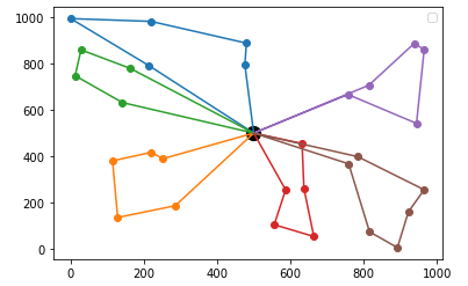
\includegraphics[width=0.5\textwidth]{Gambar/Picture1.png}
  \caption{Solusi MTSP dengan membagi menjadi 6 klaster}
  \label{fig:mtsp6}
\end{figure}

\begin{figure}[H]
  \centering
  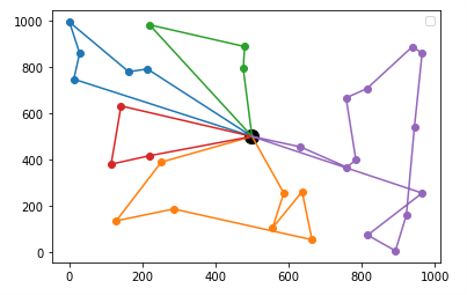
\includegraphics[width=0.5\textwidth]{Gambar/Picture2.png}
  \caption{Solusi MTSP dengan membagi menjadi 5 klaster}
  \label{fig:mtsp5}
\end{figure}

\subsection{Algoritma}

Maulana menyebutkan dalam artikelnya algoritma adalah kumpulan perintah untuk menyelesaikan suatu masalah dan diselesaikan dengan cara sistematis, terstruktur dan logis \cite{maulana2017pembelajaran}. Algoritma digunakan untuk memcahkan permasalahan yang dialami oleh seorang pengguna program.

\subsection{Algoritma $k$-means}

$K$-Means adalah jenis metode klasifikasi tanpa pengawasan yang mempartisi item data menjadi satu atau lebih klaster \cite{agusta2007k}. $K$-Means mencoba untuk memodelkan suatu dataset ke dalam beberapa klaster sehingga item-item data dalam suatu klaster memiliki karakteristik yang sama dan memiliki karakteristik yang berbeda dengan klaster lainnya.

Menurut S Monalisa \cite{monalisa2018klasterisasi} tahapan mengklaster menggunakan algoritma \textit{k}-means adalah sebagai berikut.

\begin{enumerate}
	\item Menentukan banyak klaster
	\item Memilih beberapa \textit{centroid} secara acak sesuai banyak klaster
	\item Hitung jarak titik ke centroid dengan rumus \textit{euclidean distance} seperti Persamaan (\ref{eq:euclidean1}).
	\begin{equation}
	d_{xy}=\sqrt{\sum_{i=1}^{n}(x_i-y_i)^{2}}
	\label{eq:euclidean1}
	\end{equation}
	\item Titik-titik yang tersebar masuk ke klaster yang sama dengan titik \textit{centroid} yang paling dekat
	\item Perbarui \textit{centroid} dengan menghitung nilai rata-rata nilai pada masing-masing klaster
	\item Lakukan iterasi sebanyak mungkin dengan kembali ke tahapan 3 sampai tidak ada perubahan klaster atau perubahan nilai \textit{centroid}
\end{enumerate}


\subsection{Algoritma Genetika}

Pada artikel Hermanto disebutkan bahwa algoritma genetika adalah algoritma yang digunakan untuk mencari solusi suatu permasalahan dengan cara yang lebih alami yang terispirasi dari teori evolusi  \cite{hermawanto2003algoritma}. Dalam hal ini, algoritma genetika dapat juga digunakan untuk pencarian sebuah rute terpendek dalam sebuah kasus perjalanan.

Menurut Armanda RS \cite{armanda2016penerapan} dalam artikelnya menyampaikan penyelesaian masalah menggunakan algoritma genetika memerlukan beberapa tahapan sebagai berikut:

\begin{enumerate}
	\item Menyiapkan populasi, dalam penelitian ini yang digunakan adalah data yang telah diklaster menggunakan algoritma \textit{k}-means
	\item Melakukan reproduksi dengan \textit{crossover} dan mutasi pada pembentukan awal populasi
	\item Seleksi dengan metode elitism
	\item Menentukan nilai fitness agar mendapatkan solusi akhir yang optimal
	\item Iterasi dilakukan untuk generasi berikutnya.
\end{enumerate}

\subsection{Fitness}
Fitness adalah suatu ukuran yang dijadikan acuan untuk mengetahui baik atau tidaknya suatu individu atau bisa disebut nilai dari fungsi tujuan \cite{basuki2003strategi}. Tujuan dari penggunaan algoritma genetika adalah untuk mengoptimalkan nilai fitness dengan cara mencari nilai fitness yang paling maksimal atau minimal. Seperti dalam penelitian ini yang tujuannya adalah mencari jarak yang paling minimal maka nilai fitness nya yang dicari adalah yang paling minimal juga.

\subsection{\textit{Crossover}}
\textit{Crossover} atau persilangan adalah operator dari algoritma genetika yang melibatkan dua induk untuk membentuk kromosom baru menurut artikel \cite{hardi2014analisis}. Dalam langkah ini dilakukan dengan cara menukar sebagian gen pada kromosom induk pertama dengan gen pada kromosom induk kedua seperti pada Gambar \ref{fig:crossover}. Proses \textit{crossover} tersebut diterapkan pada setiap individu dengan probabilitas \textit{crossover} ($p_c$) yang telah ditentukan. Jika diterapkan \textit{crossover} keturunan didapatkan dari kromosom-kromosom induk. Namun jika \textit{crossover} tidak diterapkan satu induk dipilih secara random dengan $p_c$ yang sama dan diduplikasi menjadi anak.

\begin{figure}[H]
  \centering
  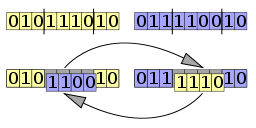
\includegraphics[width=0.5\textwidth]{Gambar/crossover.png}
  \caption{Proses crossover}
  \label{fig:crossover}
\end{figure}

\subsection{Mutasi}
Mutasi atau mutation adalah operator yang digunakan untuk mengubah gen-gen yang terdapat dalam kromosom. Model dalam proses ini sebagaimana yang terjadi dalam kehidupan alam \cite{rovie2014genetic} seperti pada Gambar \ref{fig:mutasi}. Dalam proses mutasi akan dibangkitkan sebuah bilangan random sebagai Probabilitas mutasi ($p_m$) yang sangat kecil. Mutasi diterapkan dengan tujuan untuk memperoleh nilai fitness yang lebih baik dari sebelumnya, dan lama-kelamaan akan menjadi solusi optimum yang diinginkan.

\begin{figure}[H]
  \centering
  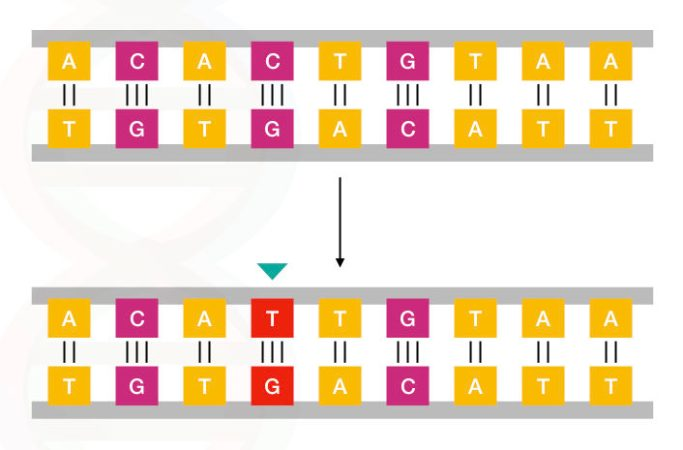
\includegraphics[width=0.5\textwidth]{Gambar/mutasi.jpg}
  \caption{Proses mutasi}
  \label{fig:mutasi}
\end{figure}

\chapter{METODE PENELITIAN}
\section{Model Penelitian dan Pengembangan}

\textit{Research and Development (R\&D)} atau penelitian dan pengembangan adalah suatu metode penelitian yang digunakan untuk menghasilkan produk tertentu, dan menguji keefektifan produk \cite{sugiyono2013metode}. 
Berdasarkan pendapat tersebut, metode \textit{Research and Development (R\&D)} atau penelitian dan pengembangan dalam bidang pendidikan merupakan penelitian yang bertujuan untuk menghasilkan atau mengembangkan dan menvalidasi suatu produk pendidikan secara efektif.
Model penelitian dan pengembangan dalam skripsi ini melalui tahapan sebagai berikut.

\begin{enumerate}
	\item Tahap pengumpulan data, kegiatan yang dilakukan pada tahap pertama adalah peneliti mengumpulkan data. Pada tahap ini peneliti juga mencari informasi data, yaitu membaca artikel penelitian sebelumnya yang berkaitan dan juga menyiapkan alat bantu atau aplikasi yang akan digunakan untuk membantu pengolahan data. Dari tahap ini data akan dikumpulkan untuk kemudian melanjutkan ke tahapan selanjutnya.
	\item Tahap pengolahan data, pada tahap ini penulis mulai mengolah data yang telah dikumpulkan sebelumnya untuk di olah dan dari tahap ini akan dilakukan ujicoba untuk mengetahui keefektifan suatu produk.
	\item Tahap analisis, setelah mendapatkan hasil uji coba peneliti mulai menganalisis hasil, menjabarkan, serta mengevaluasinya.
	\item Tahap implementasi, pada tahap terakhir ini penelitian yang telah dievaluasi dapat digunakan dan diterapkan pada tempat penelitian.
\end{enumerate}
\section{Prosedur Penelitian dan Pengembangan}


\subsection{Data Penelitian}
    
Berdasarkan studi kasus dalam skripsi ini, data yang akan digunakan dalam penelitian ini adalah data koordinat dari seluruh SMA di Kabupaten Probolinggo. Data nama-nama sekolah dikumpulkan dari \url{https://referensi.data.kemdikbud.go.id/} \cite{kemendikbud}, dan data koordinat dikumpulkan melalui aplikasi Google Earth yang dapat diunduh langsug ke dalam bentuk spreadsheet, dapat dilihat pada Lampiran \ref{lampiran1}. Waktu yang diperlukan peneliti untuk mengumpulkan data dari web tersebut kurang lebih sekitar satu bulan.

\subsection{Instrumen Pendukung}
\begin{enumerate}
    \item Python
    
    Dalam penelitian ini akan digunakan bahasa pemrograman python untuk mempermudah pengerjaan. Bahasa python adalah bahasa pemrograman baru di masa sekarang, karena dalam bahasa ini lebih simple dan singkat dalam membuat program \cite{syahrudin2018input}. Bahasa pemrograman ini merupakan bahasa pemrograman yang paling mudah dipelajari dari pada bahasa pemrograman yang lain. Serta dalam bahasa pemrograman ini dapat menjalankan beberapa rumus matematika di dalamnya. Selain itu bahasa Python telah digunakan secara luas, dan masuk dalam 3 besar bahasa pemrograman yang digunakan dalam beberapa tahun belakangan.
    
    \item Jupyter Notebook
    
    Jupyter Notebook adalah aplikasi web gratis yang digunakan untuk membuat dan membagikan dokumen komputasi, hasil hitungan, visualisasi, dan teks \cite{Kluyver2016jupyter}. Notebook ini juga mendukung 3 bahasa pemrograman salah satunya adalah bahasa pemrograman python. Banyak kelebihan yang disajikan dari aplikasi ini salah satunya adalah mendokumentasikan kode, dan menjalankan kode dalam setiap sel, dan visualisasi data seperti pada Gambar \ref{fig:visjupyter}.

\begin{figure}[H]
  \centering
  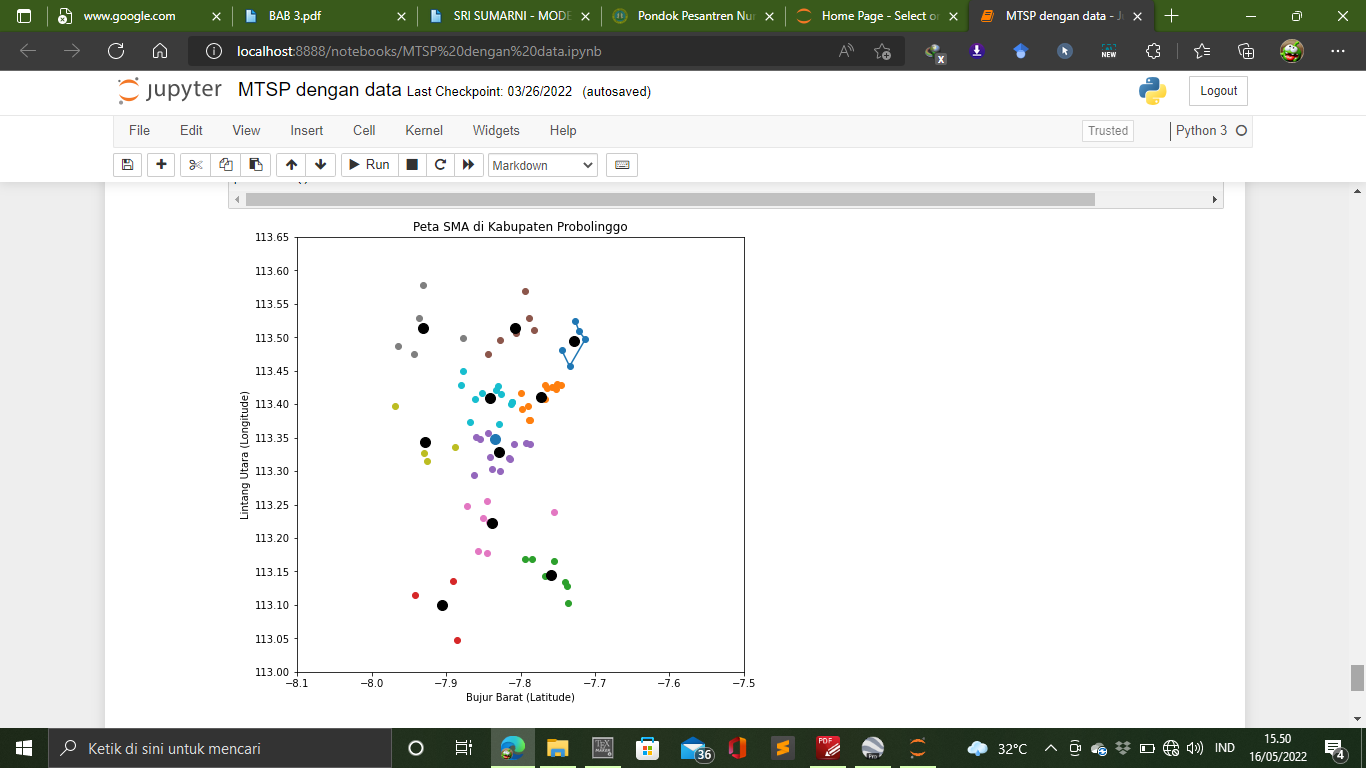
\includegraphics[width=0.8\textwidth]{Gambar/visualisasi jupyter.png}
  \caption{Visualisasi data jupyter notebook}
  \label{fig:visjupyter}
\end{figure}

	\item Google Earth
	
	Google Earth digunakan dalam penelitian ini untuk mengumpulkan koordinat lokasi seluruh SMA di Kabupaten Probolinggo. Aplikasi ini dapat menandai beberapa lokasi secara langsung seperti pada Gambar \ref{fig:markloc} dan mengekspor kedalam bentuk spreadsheet seperti pada Gambar \ref{fig:eksspread}. Data-data lokasi yang telah didownload ke dalam bentuk spreadsheet akan diproses menggunakan jupyter notebook.

\begin{figure}[H]
  \centering
  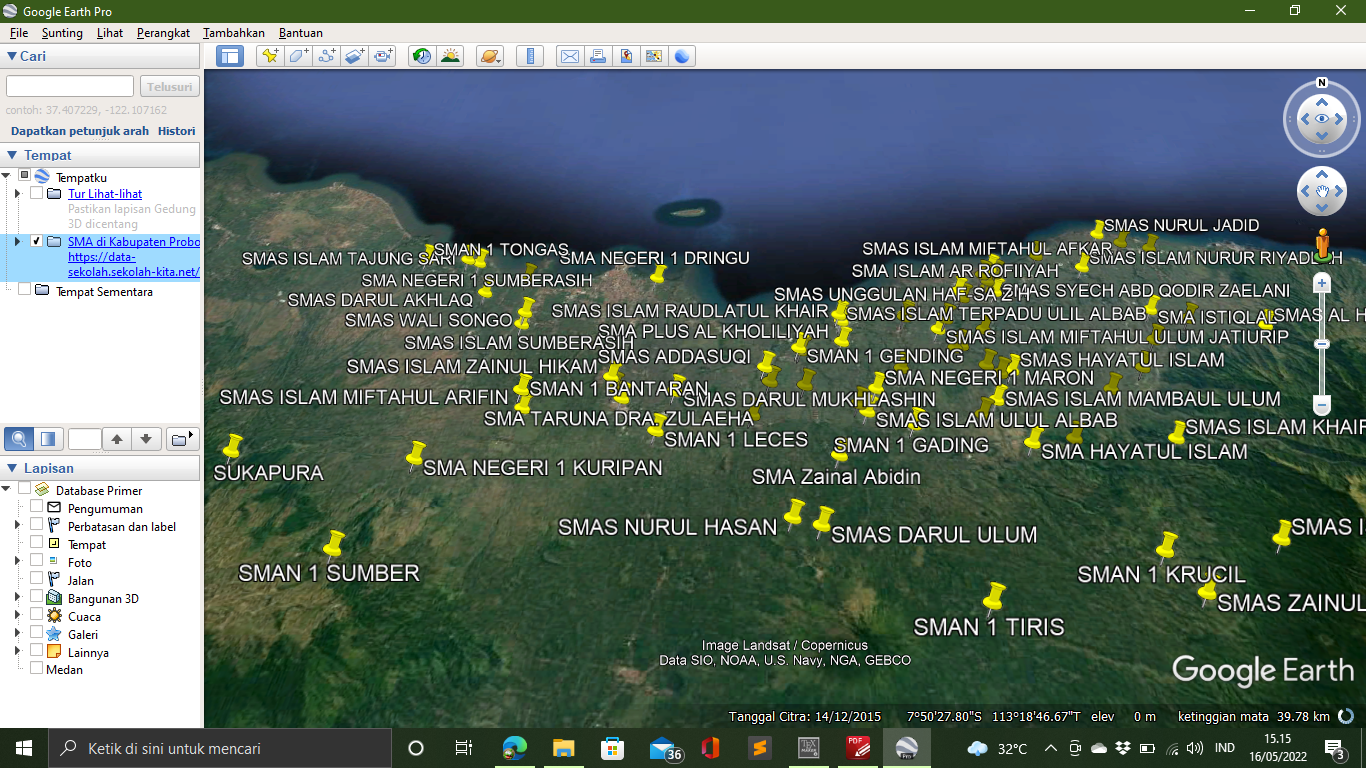
\includegraphics[width=0.8\textwidth]{Gambar/google earth.png}
  \caption{Menandai lokasi pada Google Earth}
  \label{fig:markloc}
\end{figure}

\begin{figure}[H]
  \centering
  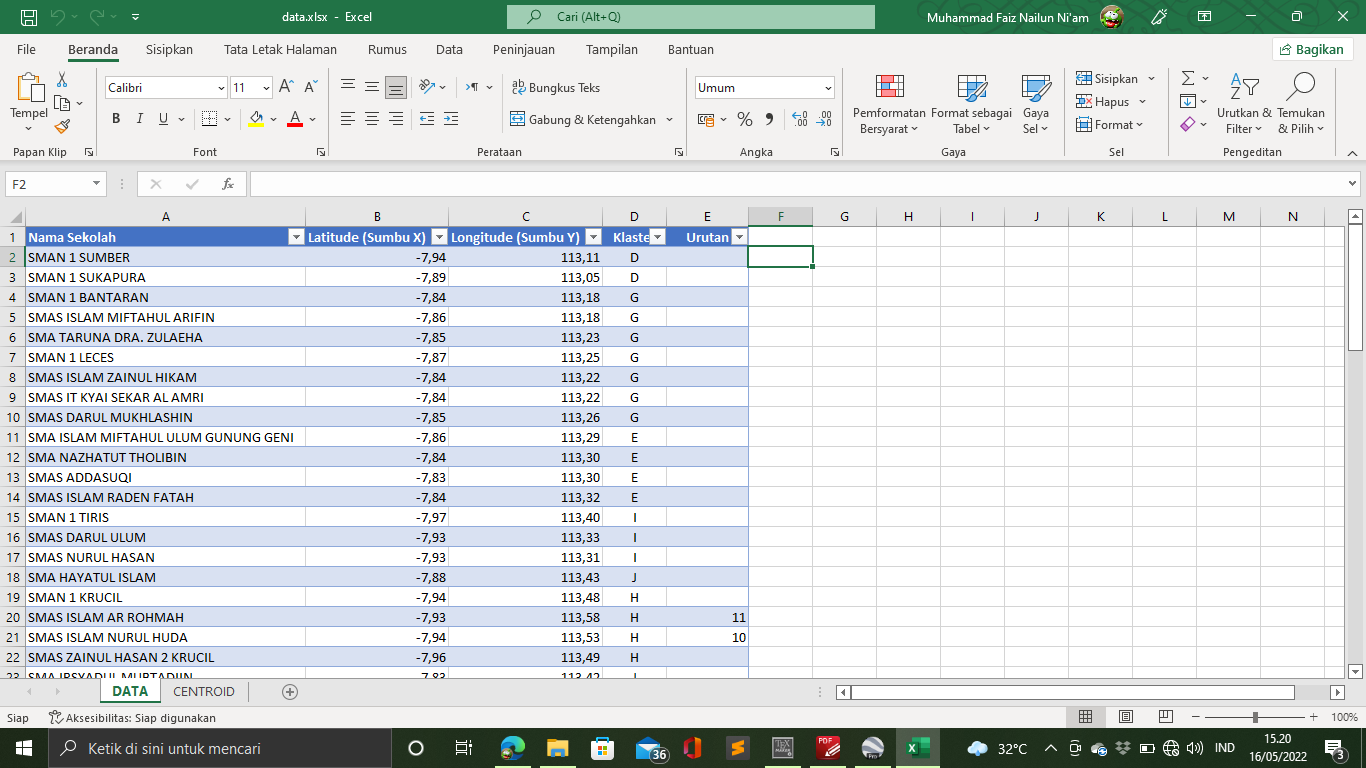
\includegraphics[width=0.8\textwidth]{Gambar/ekspor spreadsheet.png}
  \caption{Mengekspor data ke bentuk spreadsheet}
  \label{fig:eksspread}
\end{figure}

\end{enumerate}

\subsection{Langkah-langkah Dalam Tahap Pengolahan Data}
\begin{enumerate}
    \item Menyiapkan data yang telah dikumpulkan sebelumnya.
    \item Selanjutnya menentukan jumlah klaster yaitu sebanyak $n$ klaster. Data yang telah dikumupulkan pada tahap ini akan dibagi menjadi beberapa klaster, metode yang digunakan algoritma \textit{k}-means.
    \item Langkah-langkah yang digunakan dalam metode \textit{k}-means adalah sebagai berikut
    \begin{enumerate}
        \item Tentukan jumlah klaster
        \item Pilih titik-titik centroid sesuai banyak klaster
        \item \label{ulang1} Hitung jarak tiap titik tujuan dengan masing-masing \textit{centroid} dengan rumus \textit{Euclidean distance} seperti pada Persamaan (\ref{eq:euclidean}).
        \begin{equation}
        d_{xy}=\sqrt{\sum_{i=1}^{n}(x_i-y_i)^{2}}
        \label{eq:euclidean}
        \end{equation}
        \item Setelah seluruh titik masuk ke dalam klaster, hitung \textit{centroid} baru dengan cara menghitung rata-rata titik pada klaster tersebut. Lakukan hal yang sama pada klaster yang lain.
        \item Ulangi langkah \ref{ulang1} sampai tidak ada perubahan pada anggota klaster.
    \end{enumerate}
	
	\item Selanjutnya melakukan proses TSP pada setiap klaster yang telah dibagi, langkah-langkahnya adalah sebagai berikut.
	\begin{enumerate}
		\item Bangkitkan populasi awal yang berisi sejumlah kromosom
	    \item \label{ulang2} Hitung nilai \textit{fitness} (jarak) tiap kromosom
	    \item Tetapkan probabilitas \textit{crossover} ($p_c$) dan bangkitkan bilangan random (0,0000 sampai 1,0000) pada tiap kromosom, jika bilangan random kurang dari $p_c$ maka dilakukan \textit{crossover}. Jika \textit{fitness} kromosom hasil \textit{crossover} lebih baik dari kromosom awal, maka kromosom awal digantikan dengan kromosom hasil \textit{crossover}.
	    \item Tetapkan probabilitas mutasi ($p_m$) dan bangkitkan bilangan random (0,0000 sampai 1,0000) pada setiap kromosom. Jika bilangan random kurang dari $p_m$ maka akan dilakukan mutasi. Kromosom awal digantikan dengan kromosom hasil mutasi jika kromosom hasil mutasi memiliki fitness yang lebih baik dari kromosom awal.
	    \item Jika hasil kurang optimal, iterasi dilakukan dengan cara kembali ke tahapan \ref{ulang2} untuk generasi berikutnya sampai hasil yang dilakukan optimal atau mendekati optimal.
    \end{enumerate}
	\item Ketika proses diatas selesai dilakukan maka dihasilkanlah pembagian klaster dan rute terdekat tiap klaster menuju seluruh SMA di Kabupaten Probolinggo
	\item Mengevaluasi data yang dihasilkan
\end{enumerate}

\chapter{HASIL}
33\section{Penyajian Data Uji Coba}

Pada penelitian ini dilakukan uji coba menggunakan data lokasi seluruh SMA di Kabupaten Probolinggo, dan dijalankan menggunakan python. Berikut adalah sajian data hasil uji coba.

\subsection{Pengambilan Data Lokasi}

Data yang digunakan adalah data koordinat lokasi yang diekspor melalui google earth. Pengujian Pengambilan data lokasi bertujuan untuk menunjukkan bahwa sistem 
mampu membaca input yang dimasukkan. Dapat dilihat pada Lampiran \ref{lampiran1} seluruh nama-nama SMA di Kabupaten Probolinggo beserta koordinat lokasinya. Visualisasi data dari koordinat-koordinat SMA di kabupaten probolinggo dapat dilihat pada Gambar \ref{fig:petasma}.

\begin{figure}[H]
  \centering
  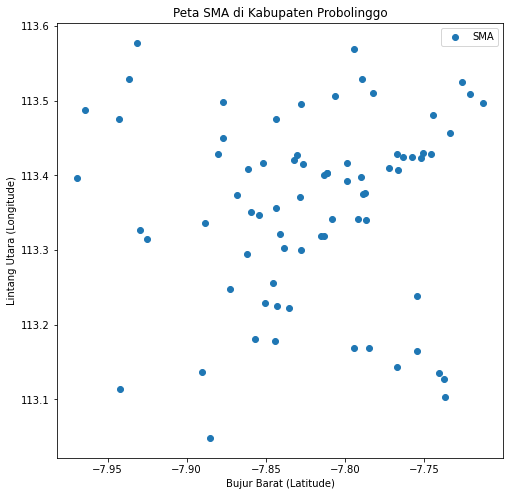
\includegraphics[width=0.5\textwidth]{Gambar/peta sma.png}
  \caption{Visualisasi lokasi SMA di Kabupaten Probolinggo}
  \label{fig:petasma}
\end{figure}

Setelah mendapatkan lokasi yang akan diproses, selanjutnya adalah menentukan beberapa titik centroid secara random, dalam penelitian ini akan diambil 8 centroid secara random seperti pada Tabel \ref{tab:dasen} dan Gambar \ref{fig:visdasen}.

\begin{table}[H]
\centering
\begin{tabular}{cccll}
\cellcolor[HTML]{4472C4}{\color[HTML]{FFFFFF} \textbf{Nama   Centroid}} & \cellcolor[HTML]{4472C4}{\color[HTML]{FFFFFF} \textbf{Latitude (Sumbu X)}} & \cellcolor[HTML]{4472C4}{\color[HTML]{FFFFFF} \textbf{Longitude (Sumbu Y)}} &  &  \\
\cellcolor[HTML]{D9E1F2}A                                               & \cellcolor[HTML]{D9E1F2}-7,81                                              & \cellcolor[HTML]{D9E1F2}113,14                                              &  &  \\
B                                                                       & -7,77                                                                      & 113,51                                                                      &  &  \\
\cellcolor[HTML]{D9E1F2}C                                               & \cellcolor[HTML]{D9E1F2}-7,77                                              & \cellcolor[HTML]{D9E1F2}113,40                                              &  &  \\
D                                                                       & -7,88                                                                      & 113,35                                                                      &  &  \\
\cellcolor[HTML]{D9E1F2}E                                               & \cellcolor[HTML]{D9E1F2}-7,93                                              & \cellcolor[HTML]{D9E1F2}113,51                                              &  &  \\
F                                                                       & -7,83                                                                      & 113,27                                                                      &  &  \\
\cellcolor[HTML]{D9E1F2}G                                               & \cellcolor[HTML]{D9E1F2}-7,84                                              & \cellcolor[HTML]{D9E1F2}113,42                                              &  & 
\end{tabular}
\caption{Koordinat titik-titik centroid pada pembagian menjadi 8 klaster}
\label{tab:dasen}
\end{table}

\begin{figure}[H]
	\centering
	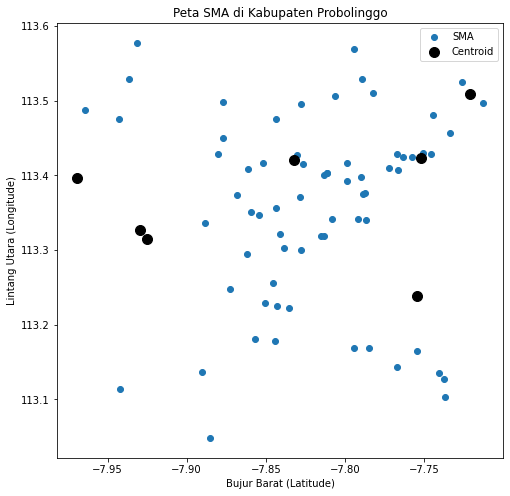
\includegraphics[width=0.5\textwidth]{Gambar/titik centroid.png}
	\caption{Visualisasi Centroid}
	\label{fig:visdasen}
\end{figure}

\subsection{Proses Pengklasteran Data}

Pada tahap ini metode yang digunakan adalah metode $K-$means untuk mengklaster data. Langkah-langkah nya adalah sebagai berikut.

\begin{enumerate}
	\item Menentukan jumlah klaster, dalam hal ini yang digunakan adalah 8 klaster.
	\item Memilih titik-titik centroid sebanyak jumlah klaster seperti pada Tabel \ref{tab:dasen} dan \ref{fig:visdasen}
	\item \label{ulang3} Hitung jarak tiap titik sekolah yang ada dengan masing-masing \textit{centroid}. Penghitungan jarak menggunakan \textit{Euclidean Distance} pada persamaan (\ref{eq:euclidean3}.
	\item Kelompokan data ke dalam klaster yang memiliki jarak paling minimum.
	\item Setelah seluruh titik sekolah masuk ke dalam klaster-klaster, hitung \textit{centroid} yang baru dengan cara menghitung rata-rata titik sekolah yang ada di dalam klaster tersebut. Lakukan hal yang sama pada klaster yang lain.
	\item Jika terdapat perubahan klaster, maka ulangi langkah \ref{ulang3} hingga tidak ada perubahan anggota pada tiap klaster. Jika \textit{centroid} yang baru tidak berubah dari sebelumnya, maka proses berhenti, karena \textit{centroid} yang tidak berubah menyebabkan anggota klaster juga tidak berubah.
	
	\begin{equation}
	\left[ \left( x,y \right) ,\left( a,b \right)\right]=\sqrt{\left( x-a \right)^{2}+\left( y-b \right)^{2}}
	\label{eq:euclidean3}
	\end{equation}
	
	\item Setelah semua data terklasifikasi, selanjutnya adalah memperbarui titik-titik centroid dengan cara menghitung rata-rata tiap anggota klaster.
\end{enumerate}

\subsection{Proses TSP menggunakan Algoritma Genetika}

Setelah data terklaster seperti pada Gambar \ref{fig:hasilklas} selanjutnya adalah mencari rute terdekatnya menggunakan Algoritma Genetika

\begin{figure}[H]
	\centering
	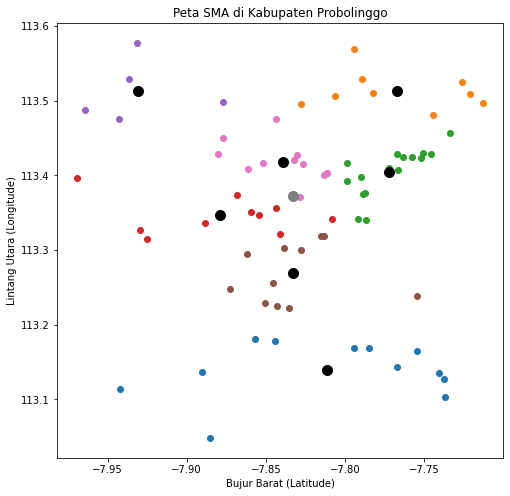
\includegraphics[width=0.5\textwidth]{Gambar/hasil klaster.png}
	\caption{Visualisasi klaster sesuai warna}
	\label{fig:hasilklas}
\end{figure}

\begin{enumerate}
	\item Bangkitkan beberapa populasi awal berisi sejumlah kromosom yang di dalamnya terdapat urutan perjalanan menuju titik sekolah.
	\item \label{ulang4} Hitung nilai \textit{fitness} (total jarak) dari tiap kromosom.
	\item Menetapkan probabilitas \textit{crossover} ($p_c$) dalam hal ini yang digunakan adalah $p_c=0,95$. Bangkitkan bilangan random (0,0000 sampai 1,0000) pada setiap kromosom, kromosom dengan bilangan random kurang dari $p_c$ maka akan dilakukan \textit{crossover}. Jika kromosom hasil \textit{crossover} memiliki \textit{fitness} yang lebih baik  dari kromosom awal, maka kromosom awal digantikan oleh kromosom hasil \textit{crossover}.
	\item Menetapkan probabilitas mutasi ($p_m$), dalam hal ini digunakan $p_m=0,1$. Bangkitakan bilangan random (0,0000 sampai 1,0000) pada setiap kromosom, kromosom yang memiliki bilangan random kuran dari $p_m$ maka akan dilakukan mutasi. Jika kromosom hasil mutasi memiliki \textit{fitness} yang lebih baik dari kromosom awal, maka kromosom awal digantikan oleh kromosom hasil mutasi.
	\item Jika hasil kurang optimal, iterasi dilakukan dengan cara kembali ke tahapan (\ref{ulang4}) untuk generasi berikutnya sampai hasil yang dilakukan optimal atau mendekati optimal.
\end{enumerate}

\subsection{Hasil dari proses \textbf{$k$}-means dan Algoritma Genetika}

Dari serangkaian proses di atas, menghasilkan beberapa rute optimal yang dapat dilalui seperti pada Gambar \ref{fig:vishasilmtsp}. Rute-rute yang dihasilkan telah diurutkan sebelumnya dan telah diekspor ke bentuk spreadsheet sehingga mempermudah pengguna dalam membaca data seperti pada Tabel \ref{tab:datahasil} merupakan urutan perjalanan pada klaster A.

\begin{figure}[H]
	\centering
	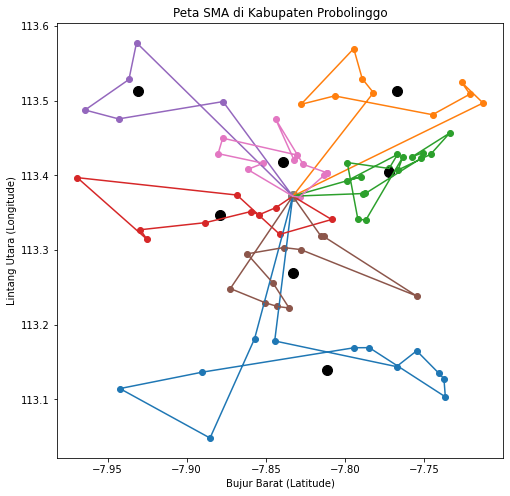
\includegraphics[width=0.5\textwidth]{Gambar/hasil mtsp.png}
	\caption{Visualisasi hasil pembagian klaster dan rute yang dapat dilalui}
	\label{fig:vishasilmtsp}
\end{figure}

\begin{table}[h!]
\begin{adjustbox}{width=\columnwidth,center}
\begin{tabular}{lllcl}
\rowcolor[HTML]{4472C4} 
\multicolumn{1}{c}{\cellcolor[HTML]{4472C4}{\color[HTML]{FFFFFF} \textbf{Nama   Sekolah}}} & \multicolumn{1}{c}{\cellcolor[HTML]{4472C4}{\color[HTML]{FFFFFF} \textbf{Latitude (Sumbu X)}}} & \multicolumn{1}{c}{\cellcolor[HTML]{4472C4}{\color[HTML]{FFFFFF} \textbf{Longitude (Sumbu Y)}}} & {\color[HTML]{FFFFFF} \textbf{Klaster}} & \multicolumn{1}{c}{\cellcolor[HTML]{4472C4}{\color[HTML]{FFFFFF} \textbf{Urutan}}} \\
\rowcolor[HTML]{D9E1F2} 
SMAS ISLAM MIFTAHUL ARIFIN                                                                 & -7,86                                                                                          & 113,18                                                                                          & A                                       & 0                                                                                  \\
SMAN   1 SUKAPURA                                                                          & -7,89                                                                                          & 113,05                                                                                          & A                                       & 1                                                                                  \\
\rowcolor[HTML]{D9E1F2} 
SMAN 1 SUMBER                                                                              & -7,94                                                                                          & 113,11                                                                                          & A                                       & 2                                                                                  \\
SMA   NEGERI 1 KURIPAN                                                                     & -7,89                                                                                          & 113,14                                                                                          & A                                       & 3                                                                                  \\
\rowcolor[HTML]{D9E1F2} 
SMAS ISLAM SUMBERASIH                                                                      & -7,79                                                                                          & 113,17                                                                                          & A                                       & 4                                                                                  \\
SMAS   WALI SONGO                                                                          & -7,78                                                                                          & 113,17                                                                                          & A                                       & 5                                                                                  \\
\rowcolor[HTML]{D9E1F2} 
SMAN 1 TONGAS                                                                              & -7,74                                                                                          & 113,10                                                                                          & A                                       & 6                                                                                  \\
SMAS   ISLAM TAJUNG SARI                                                                   & -7,74                                                                                          & 113,13                                                                                          & A                                       & 7                                                                                  \\
\rowcolor[HTML]{D9E1F2} 
SMA NEGERI 1 SUMBERASIH                                                                    & -7,74                                                                                          & 113,13                                                                                          & A                                       & 8                                                                                  \\
SMAS   ASSUBHAN                                                                            & -7,75                                                                                          & 113,16                                                                                          & A                                       & 9                                                                                  \\
\rowcolor[HTML]{D9E1F2} 
SMAS DARUL AKHLAQ                                                                          & -7,77                                                                                          & 113,14                                                                                          & A                                       & 10                                                                                 \\
SMAN   1 BANTARAN                                                                          & -7,84                                                                                          & 113,18                                                                                          & A                                       & 11                                                                                
\end{tabular}
\end{adjustbox}
\caption{Urutan perjalanan pada klaster A}
\label{tab:datahasil}
\end{table}

\subsection{Percobaan menggunakan banyak klaster yang berbeda}

Pada penelitian ini tidak hanya menggunakan pembagian 8 klaster saja, namun sebelumnya telah diuji coba menggunakan banyak klaster yang berbeda seperti pada Gambar \ref{fig:klasterbeda}. Dalam gambar tersebut telah diuji coba menggugunakan pembagian 1 klaster hingga 10 klaster, namun setelah dihitung jarak yang minimal yang dapat dilalui berada pada pembagian 8 klaster seperti Tabel \ref{tab:totaljarak} membuktikan bahwa pembagian menjadi 8 klaster dapat menghasilkan jarak yang paling minimum.

\begin{figure}[H]
	\centering
	\begin{subfigure}[b]{0.3\textwidth}
		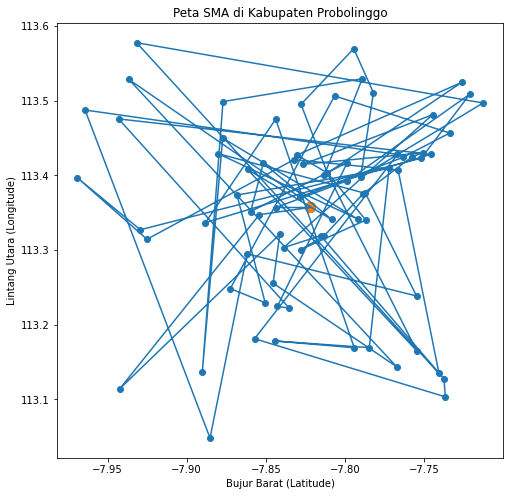
\includegraphics[width=\textwidth]{Gambar/Klaster/1.png}
		\caption{1 klaster}	
	\end{subfigure}
	\hfill
	\begin{subfigure}[b]{0.3\textwidth}
		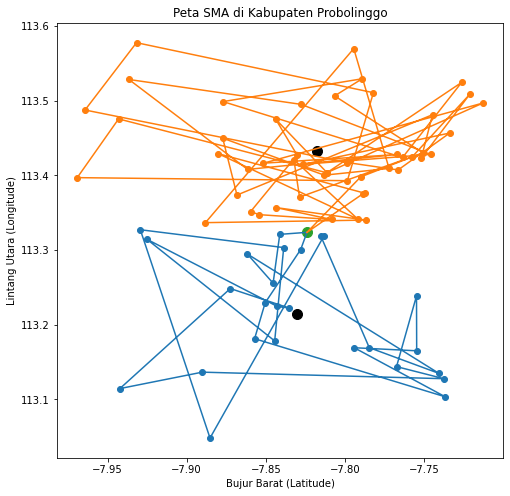
\includegraphics[width=\textwidth]{Gambar/Klaster/2.png}
		\caption{2 klaster}	
	\end{subfigure}
	\hfill
	\begin{subfigure}[b]{0.3\textwidth}
		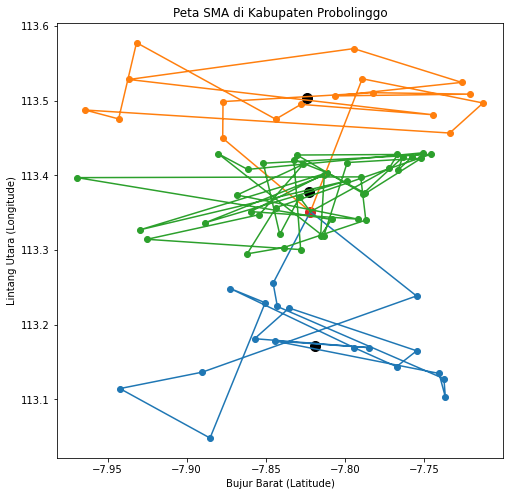
\includegraphics[width=\textwidth]{Gambar/Klaster/3.png}
		\caption{3 klaster}	
	\end{subfigure}
	\hfill
	\begin{subfigure}[b]{0.3\textwidth}
		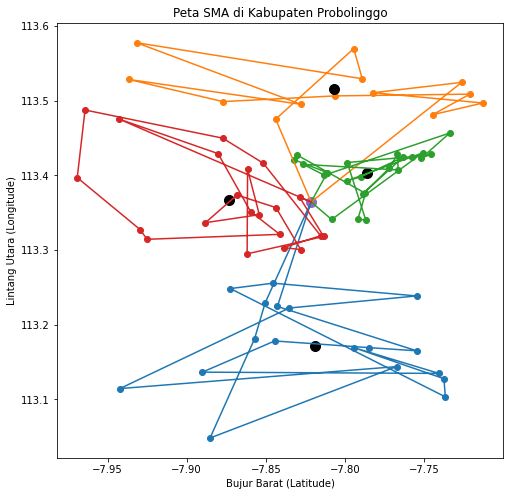
\includegraphics[width=\textwidth]{Gambar/Klaster/4.png}
		\caption{4 klaster}	
	\end{subfigure}
	\hfill
	\begin{subfigure}[b]{0.3\textwidth}
		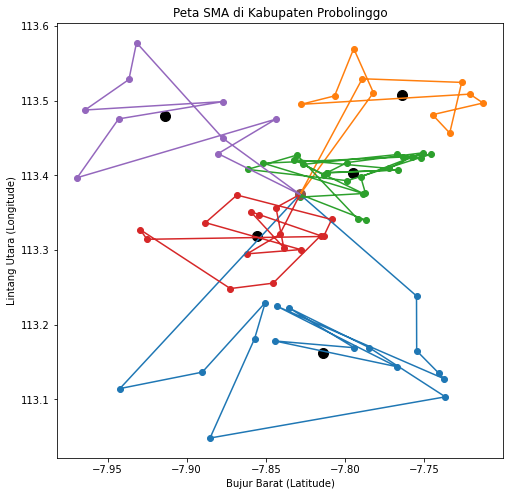
\includegraphics[width=\textwidth]{Gambar/Klaster/5.png}
		\caption{5 klaster}	
	\end{subfigure}
	\hfill
	\begin{subfigure}[b]{0.3\textwidth}
		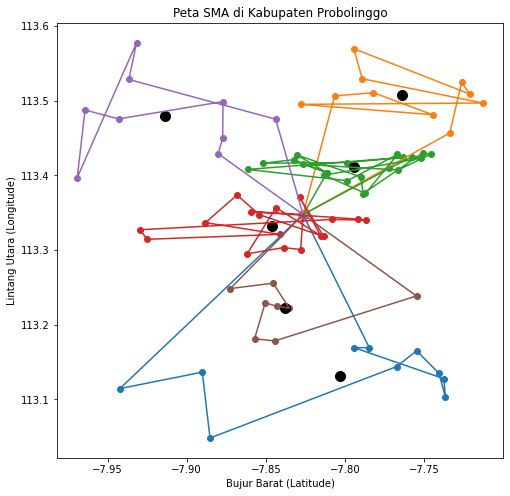
\includegraphics[width=\textwidth]{Gambar/Klaster/6.png}
		\caption{6 klaster}	
	\end{subfigure}
	\hfill
	\begin{subfigure}[b]{0.3\textwidth}
		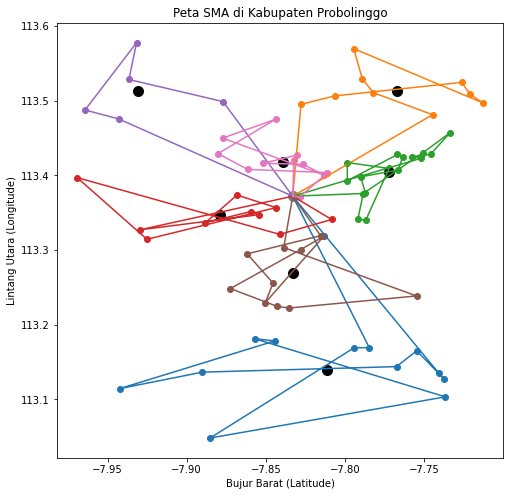
\includegraphics[width=\textwidth]{Gambar/Klaster/7.png}
		\caption{7 klaster}	
	\end{subfigure}
	\hfill
	\begin{subfigure}[b]{0.3\textwidth}
		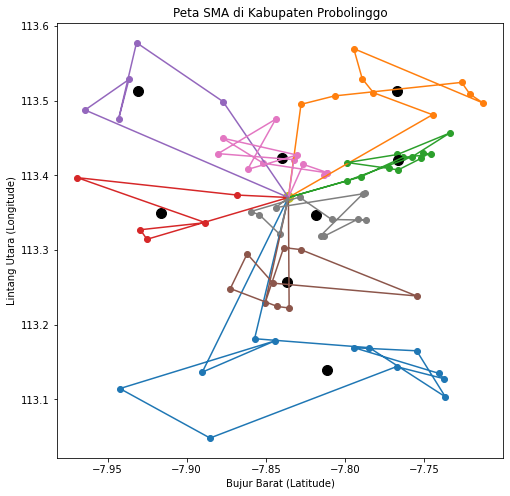
\includegraphics[width=\textwidth]{Gambar/Klaster/8.png}
		\caption{8 klaster}	
	\end{subfigure}
	\hfill
	\begin{subfigure}[b]{0.3\textwidth}
		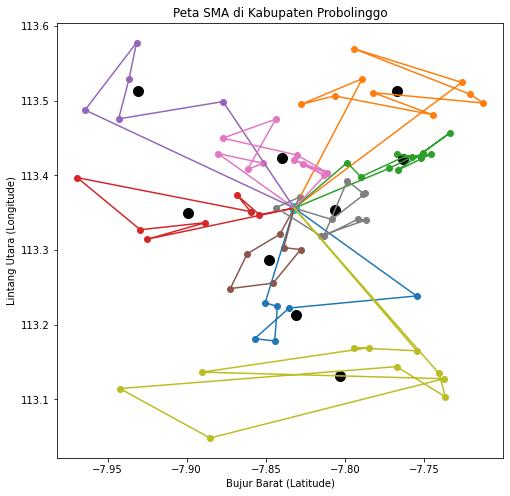
\includegraphics[width=\textwidth]{Gambar/Klaster/9.png}
		\caption{9 klaster}	
	\end{subfigure}
	\hfill
	\begin{subfigure}[b]{0.3\textwidth}
		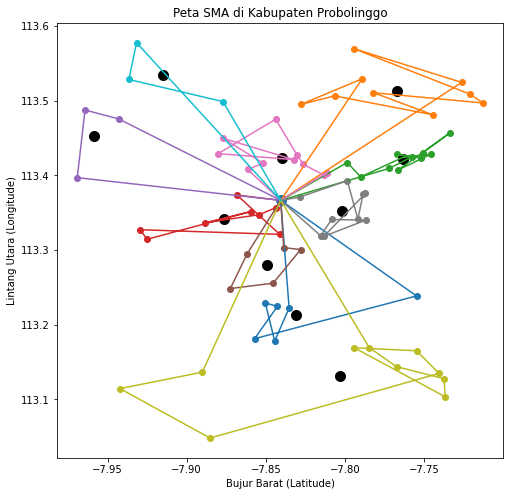
\includegraphics[width=\textwidth]{Gambar/Klaster/10.png}
		\caption{10 klaster}	
	\end{subfigure}
	\caption{Hasil rute dengan pembagian klaster berbeda}
	\label{fig:klasterbeda}
\end{figure}
\begin{table}[H]
\centering
\footnotesize
\begin{tabular}{ccccc}
\rowcolor[HTML]{4472C4} 
\cellcolor[HTML]{4472C4}{\color[HTML]{FFFFFF} } &
  \cellcolor[HTML]{4472C4}{\color[HTML]{FFFFFF} } &
  \cellcolor[HTML]{4472C4}{\color[HTML]{FFFFFF} } &
  \multicolumn{2}{c}{\cellcolor[HTML]{4472C4}{\color[HTML]{FFFFFF} \textbf{Titik Kumpul}}} \\
\rowcolor[HTML]{4472C4} 
\multirow{-2}{*}{\cellcolor[HTML]{4472C4}{\color[HTML]{FFFFFF} \textbf{Banyak Klaster}}} &
  \multirow{-2}{*}{\cellcolor[HTML]{4472C4}{\color[HTML]{FFFFFF} \textbf{Total Jarak}}} &
  \multirow{-2}{*}{\cellcolor[HTML]{4472C4}{\color[HTML]{FFFFFF} \textbf{Peringkat}}} &
  \cellcolor[HTML]{4472C4}{\color[HTML]{FFFFFF} \textbf{Latitude (X)}} &
  \cellcolor[HTML]{4472C4}{\color[HTML]{FFFFFF} \textbf{Longitude (Y)}} \\
1  & 10,0503  & 10 & -7,8221841 & 113,3570412 \\
\rowcolor[HTML]{D9E1F2} 
2  & 6,858777 & 9  & -7,8241236 & 113,3236903 \\
3  & 5,599878 & 8  & -7,8219762 & 113,3512877 \\
\rowcolor[HTML]{D9E1F2} 
4  & 5,010994 & 7  & -7,8215022 & 113,3644199 \\
5  & 4,805015 & 6  & -7,828521  & 113,3744846 \\
\rowcolor[HTML]{D9E1F2} 
6  & 4,43132  & 3  & -7,8265701 & 113,3475373 \\
7  & 4,353295 & 1  & -7,8331118 & 113,3721289 \\
\rowcolor[HTML]{D9E1F2} 
8  & 4,398984 & 2  & -7,8358502 & 113,3704048 \\
9  & 4,48243  & 4  & -7,8321462 & 113,356253  \\
\rowcolor[HTML]{D9E1F2} 
10 & 4,780413 & 5  & -7,8406976 & 113,3665328
\end{tabular}
\caption{Total jarak dengan jumlah pembagian klaster yang berbeda}
\label{tab:totaljarak}
\end{table}
%\section{Analisis Data}
%\section{Revisi Produk}

\chapter{PENUTUP}
\section{Kesimpulan}
\section{Saran}
% Daftar Pustaka
\newpage
\bibliographystyle{apalike}
\bibliography{Lain-lain/library}

\newpage
\thispagestyle{empty}
%\addcontentsline{toc}{chapter}{LAMPIRAN}
\appendix
\renewcommand{\thechapter}{\arabic{chapter}}
\renewcommand{\thesection}{\thechapter.\arabic{chapter}}
\chapter{DATASET}
\section{Nama dan Koordinat SMA di Kabupaten Probolinggo}
\label{lampiran1}

{\scriptsize
\begin{longtable}[c]{clll}
\cline{2-4}
\rowcolor[HTML]{4472C4} 
{\color[HTML]{FFFFFF} \textbf{No.}} &
  \multicolumn{1}{c}{\cellcolor[HTML]{4472C4}{\color[HTML]{FFFFFF} \textbf{Nama Sekolah}}} &
  \multicolumn{1}{c}{\cellcolor[HTML]{4472C4}{\color[HTML]{FFFFFF} \textbf{\begin{tabular}[c]{@{}c@{}}Latitude\\      (Sumbu X)\end{tabular}}}} &
  \multicolumn{1}{c}{\cellcolor[HTML]{4472C4}{\color[HTML]{FFFFFF} \textbf{\begin{tabular}[c]{@{}c@{}}Longitude\\      (Sumbu Y)\end{tabular}}}} \\ \cline{2-4} 
\endhead
%
\cline{2-4}
\endfoot
%
\endlastfoot
%
\rowcolor[HTML]{D9E1F2} 
1  & SMA DARUL HIKMAH                      & -7,76 & 113,43 \\
2  & SMA   DARUT TAQWA                     & -7,79 & 113,53 \\
\rowcolor[HTML]{D9E1F2} 
3  & SMA HAYATUL ISLAM                     & -7,88 & 113,43 \\
4  & SMA   IRSYADUL MUBTADIIN              & -7,83 & 113,42 \\
\rowcolor[HTML]{D9E1F2} 
5  & SMA ISLAM AR ROFIIYAH                 & -7,77 & 113,41 \\
6  & SMA   ISLAM MIFTAHUL ULUM GUNUNG GENI & -7,86 & 113,29 \\
\rowcolor[HTML]{D9E1F2} 
7  & SMA ISLAM SYARIF HIDAYATULLAH         & -7,81 & 113,51 \\
8  & SMA   ISTIQLAL                        & -7,78 & 113,51 \\
\rowcolor[HTML]{D9E1F2} 
9  & SMA NAZHATUT THOLIBIN                 & -7,84 & 113,30 \\
10 & SMA   NEGERI 1 DRINGU                 & -7,75 & 113,24 \\
\rowcolor[HTML]{D9E1F2} 
11 & SMA NEGERI 1 KURIPAN                  & -7,89 & 113,14 \\
12 & SMA   NEGERI 1 MARON                  & -7,84 & 113,36 \\
\rowcolor[HTML]{D9E1F2} 
13 & SMA NEGERI 1 SUMBERASIH               & -7,74 & 113,13 \\
14 & SMA   NEGERI 2 KRAKSAAN               & -7,73 & 113,46 \\
\rowcolor[HTML]{D9E1F2} 
15 & SMA PLUS AL KHOLILIYAH                & -7,81 & 113,34 \\
16 & SMA   SIROJUL ARIFIN                  & -7,80 & 113,42 \\
\rowcolor[HTML]{D9E1F2} 
17 & SMA TARUNA DRA. ZULAEHA               & -7,85 & 113,23 \\
18 & SMA   TERPADU DARUT TAUHID            & -7,81 & 113,40 \\
\rowcolor[HTML]{D9E1F2} 
19 & SMA UNGGULAN BADRIDDUJA               & -7,75 & 113,42 \\
20 & SMA   Zainal Abidin                   & -7,89 & 113,34 \\
\rowcolor[HTML]{D9E1F2} 
21 & SMAN 1 BANTARAN                       & -7,84 & 113,18 \\
22 & SMAN 1   BESUK                        & -7,83 & 113,50 \\
\rowcolor[HTML]{D9E1F2} 
23 & SMAN 1 GADING                         & -7,87 & 113,37 \\
24 & SMAN 1   GENDING                      & -7,81 & 113,32 \\
\rowcolor[HTML]{D9E1F2} 
25 & SMAN 1 KRAKSAAN                       & -7,76 & 113,42 \\
26 & SMAN 1   KRUCIL                       & -7,94 & 113,48 \\
\rowcolor[HTML]{D9E1F2} 
27 & SMAN 1 LECES                          & -7,87 & 113,25 \\
28 & SMAN 1   PAITON                       & -7,72 & 113,51 \\
\rowcolor[HTML]{D9E1F2} 
29 & SMAN 1 SUKAPURA                       & -7,89 & 113,05 \\
30 & SMAN 1   SUMBER                       & -7,94 & 113,11 \\
\rowcolor[HTML]{D9E1F2} 
31 & SMAN 1 TIRIS                          & -7,97 & 113,40 \\
32 & SMAN 1   TONGAS                       & -7,74 & 113,10 \\
\rowcolor[HTML]{D9E1F2} 
33 & SMAS ADDASUQI                         & -7,83 & 113,30 \\
34 & SMAS AL   HASYIMI                     & -7,79 & 113,57 \\
\rowcolor[HTML]{D9E1F2} 
35 & SMAS AL KHAIRIYAH                     & -7,75 & 113,43 \\
36 & SMAS   ASSUBHAN                       & -7,75 & 113,16 \\
\rowcolor[HTML]{D9E1F2} 
37 & SMAS DARUL AKHLAQ                     & -7,77 & 113,14 \\
38 & SMAS   DARUL MUKHLASHIN               & -7,85 & 113,26 \\
\rowcolor[HTML]{D9E1F2} 
39 & SMAS DARUL ULUM                       & -7,93 & 113,33 \\
40 & SMAS   HAYATUL ISLAM                  & -7,83 & 113,43 \\
\rowcolor[HTML]{D9E1F2} 
41 & SMAS IHYAUL IMAN                      & -7,88 & 113,45 \\
42 & SMAS   ISLAM AR ROHMAH                & -7,93 & 113,58 \\
\rowcolor[HTML]{D9E1F2} 
43 & SMAS ISLAM IRTIQOIYAH                 & -7,79 & 113,40 \\
44 & SMAS   ISLAM KHAIRIYAH                & -7,88 & 113,50 \\
\rowcolor[HTML]{D9E1F2} 
45 & SMAS ISLAM MAMBAUL ULUM               & -7,85 & 113,42 \\
46 & SMAS   ISLAM MIFTAHUL AFKAR           & -7,75 & 113,43 \\
\rowcolor[HTML]{D9E1F2} 
47 & SMAS ISLAM MIFTAHUL ARIFIN            & -7,86 & 113,18 \\
48 & SMAS   ISLAM MIFTAHUL ULUM JATIURIP   & -7,80 & 113,39 \\
\rowcolor[HTML]{D9E1F2} 
49 & SMAS ISLAM MIFTAHUL ULUM OPO OPO      & -7,83 & 113,41 \\
50 & SMAS   ISLAM NURUL HUDA               & -7,94 & 113,53 \\
\rowcolor[HTML]{D9E1F2} 
51 & SMAS ISLAM NURUR RIYADLAH             & -7,74 & 113,48 \\
52 & SMAS   ISLAM RADEN FATAH              & -7,84 & 113,32 \\
\rowcolor[HTML]{D9E1F2} 
53 & SMAS ISLAM RAUDLATUL KHAIR            & -7,79 & 113,34 \\
54 & SMAS   ISLAM SIROJUL UMMAH            & -7,84 & 113,48 \\
\rowcolor[HTML]{D9E1F2} 
55 & SMAS ISLAM SUMBERASIH                 & -7,79 & 113,17 \\
56 & SMAS   ISLAM TAJUNG SARI              & -7,74 & 113,13 \\
\rowcolor[HTML]{D9E1F2} 
57 & SMAS ISLAM TERPADU ULIL ALBAB         & -7,79 & 113,34 \\
58 & SMAS   ISLAM ULUL ALBAB               & -7,86 & 113,35 \\
\rowcolor[HTML]{D9E1F2} 
59 & SMAS ISLAM ZAINUL HIKAM               & -7,84 & 113,22 \\
60 & SMAS IT   KYAI SEKAR AL AMRI          & -7,84 & 113,22 \\
\rowcolor[HTML]{D9E1F2} 
61 & SMAS MIFTAHUL HASANAIN                & -7,81 & 113,40 \\
62 & SMAS   MUHAMMAD SHODIQ                & -7,83 & 113,37 \\
\rowcolor[HTML]{D9E1F2} 
63 & SMAS MUHAMMADIYAH 3 PROBOLINGGO       & -7,82 & 113,32 \\
64 & SMAS   NURUL HASAN                    & -7,93 & 113,31 \\
\rowcolor[HTML]{D9E1F2} 
65 & SMAS NURUL IMAN                       & -7,86 & 113,41 \\
66 & SMAS   NURUL JADID                    & -7,71 & 113,50 \\
\rowcolor[HTML]{D9E1F2} 
67 & SMAS SA ADAH NIZHAMUL ISLAM           & -7,85 & 113,35 \\
68 & SMAS   SYECH ABD QODIR ZAELANI        & -7,77 & 113,43 \\
\rowcolor[HTML]{D9E1F2} 
69 & SMAS TAMAN MADYA                      & -7,77 & 113,41 \\
70 & SMAS   TUNAS LUHUR                    & -7,73 & 113,52 \\
\rowcolor[HTML]{D9E1F2} 
71 & SMAS UNGGULAN HAF-SA Z H              & -7,79 & 113,38 \\
72 & SMAS   WALI SONGO                     & -7,78 & 113,17 \\
\rowcolor[HTML]{D9E1F2} 
73 & SMAS ZAINUL HASAN 1                   & -7,79 & 113,38 \\
74 & SMAS   ZAINUL HASAN 2 KRUCIL          & -7,96 & 113,49 \\
\rowcolor[HTML]{D9E1F2} 
75 & SMASI NURUL HIDAYAH                   & -7,81 & 113,40 \\ \cline{2-4} 
\caption{Daftar nama-nama SMA di Kabupaten Probolinggo}
\end{longtable}
}

%\newpage
%\thispagestyle{empty}
%\section*{Lampiran 2 Instrumen Penelitian}

%\begin{enumerate}
%\item Jupyter Notebook

%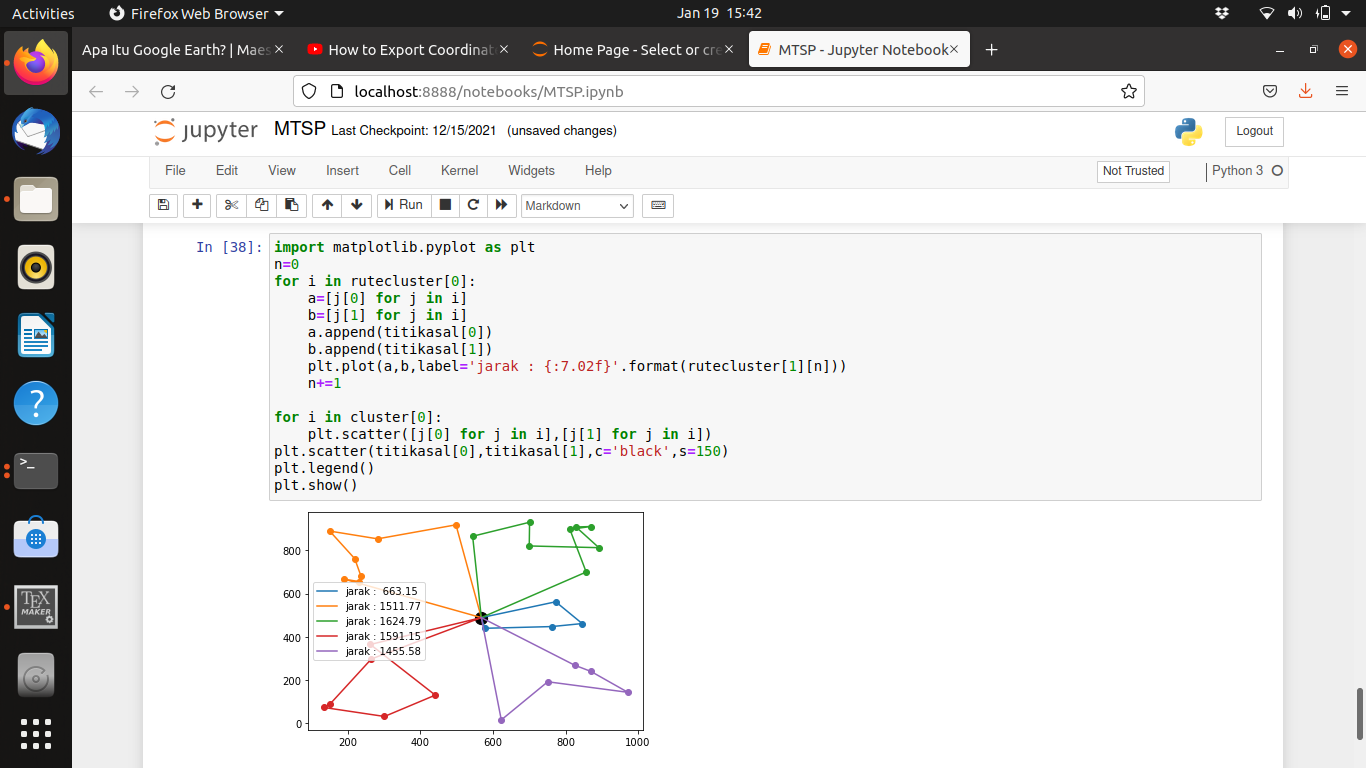
\includegraphics[width=13cm]{instrumen2.png}

%\item Google Earth

%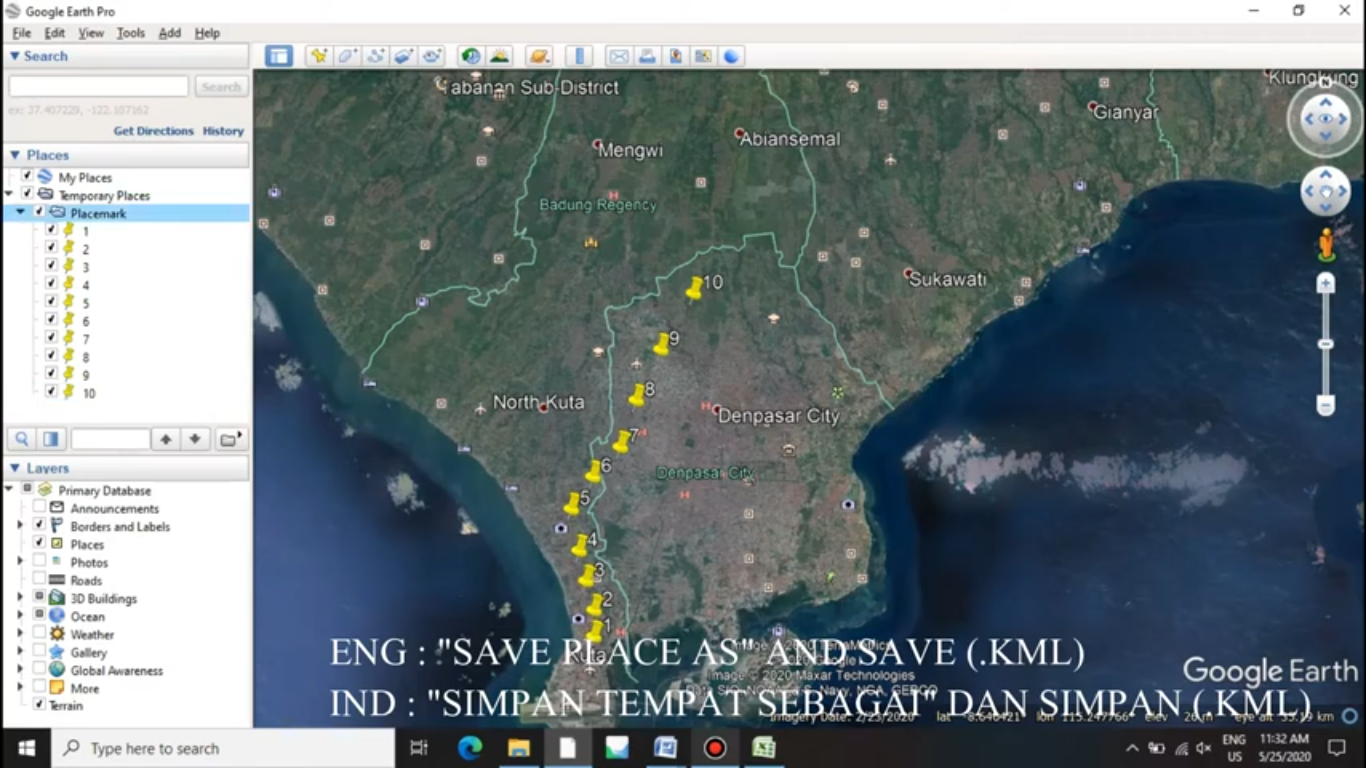
\includegraphics[width=13cm]{instrumen1.png}

%\end{enumerate}

\newpage
%\addcontentsline{toc}{chapter}{RIWAYAT HIDUP}
\chapter*{RIWAYAT HIDUP}

\noindent
\begin{wrapfigure}{l}{3cm}
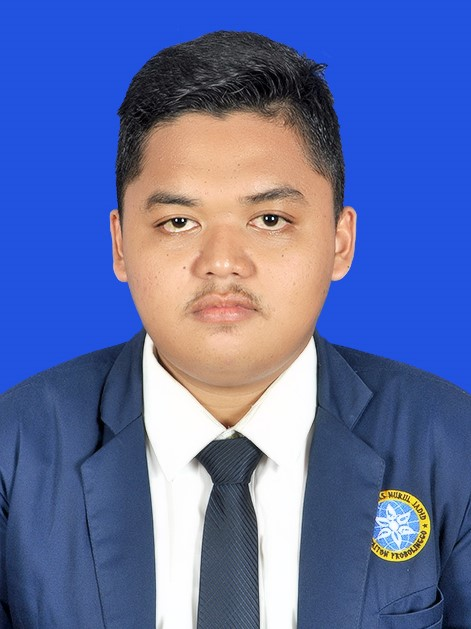
\includegraphics[width=3cm, height=4cm]{Gambar/pas foto.jpg} 
\end{wrapfigure}

Muhammad Faiz Nailun Ni'am, dilahirkan di Kabupaten Bondowoso tepatnya di Desa Tegal Mijin pada hari Rabu tanggal 12 Januari 2000. Anak pertama dari tiga bersaudara, terlahir dari pasangan Abdul Hadi dan Hosni. Peneliti menyelesaikan pendidikan Sekolah Dasar di SD Negeri Tegal Mijin 1 di Kecamatan Grujugan Kabupaten Bondowoso pada tahun 2012. Pada tahun itu juga peneliti melanjutkan Pendidikan di SMP Negeri 1 Jambesari Darussholah Kecamatan Jambesari Kabupaten Bondowoso dan selesai pada tahun 2015, kemudian melanjutkan Sekolah Menengah Atas di pesantren yaitu SMA Nurul Jadid yang berada di Pondok Pesantren Nurul Jadid Kecamatan Paiton Kabupaten Probolinggo dan selesai pada tahun 2018. Pada saat SMA peneliti mendapat berpengalaman meraih juara 2 di bidang matematika pada Kompetisi Sains Nalaria Realistik (KSNR) tingkat kabupaten pada tahun 2015 serta juara 2 di bidang informatika pada Olimpiade Sains Nasional (OSN) tingkat kabupaten pada tahun 2016.

Pada tahun 2018 peneliti melanjutkan pendidikan di perguruan tinggi swasta, tepatnya di Universitas Nurul Jadid Program Studi Pendidikan Matematika. Pengalaman saat di Universitas peneliti pernah menjadi Sekretaris Himaprodi Pendidikan Matematika Masa Bakti 2020/2021, anggota dan tenaga pengajar Bimbingan Belajar PCC Math (Personal Computer Community Of Mathematic). Peneliti pernah menjadi asisten dosen mata kuliah Pengantar Dasar Komputer Pada Februari sampai Juni 2021 di Pendidikan Matematika. Pada maret sampai april 2022 Peneliti menjadi pembimbing dalam pengabdian bersama dosen dalam pembinaan KSN Informatika Tahun 2022 di SMA Tunas Luhur Paiton Probolinggo. Selain itu peneliti juga pernah berprofesi sebagai asisten guru di MA Nurul Jadid Kecamatan Paiton Kabupaten Probolinggo. 
\end{document}